\documentclass[11pt]{beamer}

\usetheme{metropolis}

\usepackage{graphicx}
\usepackage{physics}
\usepackage{adjustbox}
\usepackage{caption}
\usepackage{chemformula}
\usepackage{quoting}
\usepackage[style=chem-angew,backend=bibtex]{biblatex}
\bibliography{references}
%
% Choose how your presentation looks.
%
% For more themes, color themes and font themes, see:
% http://deic.uab.es/~iblanes/beamer_gallery/index_by_theme.html
%
\mode<presentation>
{
  \usetheme{default}      % or try Darmstadt, Madrid, Warsaw, ...
  \usecolortheme{default} % or try albatross, beaver, crane, ...
  \usefonttheme{default}  % or try serif, structurebold, ...
  \setbeamertemplate{navigation symbols}{}
  \setbeamertemplate{caption}[numbered]
  \setbeamerfont{footnote}{size=\tiny}
} 

\usepackage[english]{babel}
\usepackage[utf8]{inputenc}
\graphicspath{{../lectureMW/image/}}

\AtBeginSection[]{
\begin{frame}{Outline}
  \tableofcontents[currentsection]
\end{frame}
}

\title{Chapter 6: Quantities in Chemical Reactions}
\institute{Chemistry Department, Cypress College}
\date{October 10, 2022}

\begin{document}

\begin{frame}
  \titlepage
\end{frame}

\begin{frame}{Class Annoucements}
  
  \textbf{Lecture}
  \begin{itemize}
  \item Finally graded homework 3 and go over homework 4 (EC for
    students who present)
  \item Finish up Ch 6 and worksheet 7; begin discussion on Ch 7
    - Electronic Structure of the Atom
  \item Quiz and Homework assignment released Fri, Oct 14th at 3pm
  \end{itemize}
\end{frame}

\section{Review: Chemical Equations. Limiting Reagent and Percent Yield}

\begin{frame}{Meaning of a Balanced Equation}
  \textbf{Photosysnthesis Chemical Equation}
  \begin{equation}
    6\text{CO$_2$(g)} + 6\text{H$_2$O(l)} \rightarrow \text{C$_6$H$_{12}$O$_6$(s)}
    + 6\text{O$_2$(g)}
  \end{equation}
  
  \begin{itemize}
  \item Balanced chemical equation satisfies the conservation of mass
  \item Coefficients in front of the molecules represent the relative
    moles of reactants and products
  \end{itemize}
\end{frame}

\begin{frame}{Approaching Limiting Reactant Problems}
  \begin{equation}
    \text{R1} + \text{R2} \rightarrow \text{P1}
  \end{equation}
  \begin{itemize}
  \item Given a certain amount of each reagents (R1 and R2)
    to produce P1, determine
    how much the R2 is needed to completely react with R1
  \item Based on that calculated value, determine whether
    there is enough R2 to completely react with R1
  \item If the amount of R2 is less than what is needed,
    then R2 is the limiting
  \item If the amount of R2 is more than what is needed,
    then R2 is the excess
  \end{itemize}
\end{frame}

\begin{frame}{Percent Yield, Theoretical Yield, and Actual}
  \textbf{Percent Yield} - describes how much product has been
  produced
  \begin{equation}
    \% = \frac{\text{actual yield}}{\text{theoretical yield}} \times 100\%
  \end{equation}
 
  \textbf{Actual Yield} - the amount produced in the lab (potential errors)

  \textbf{Theoretical Yield} - the maximum amount predicted from a given amount
  of reagents
\end{frame}

\section{Energy Changes}

\begin{frame}{Global Energy Consumption}
  \centering
  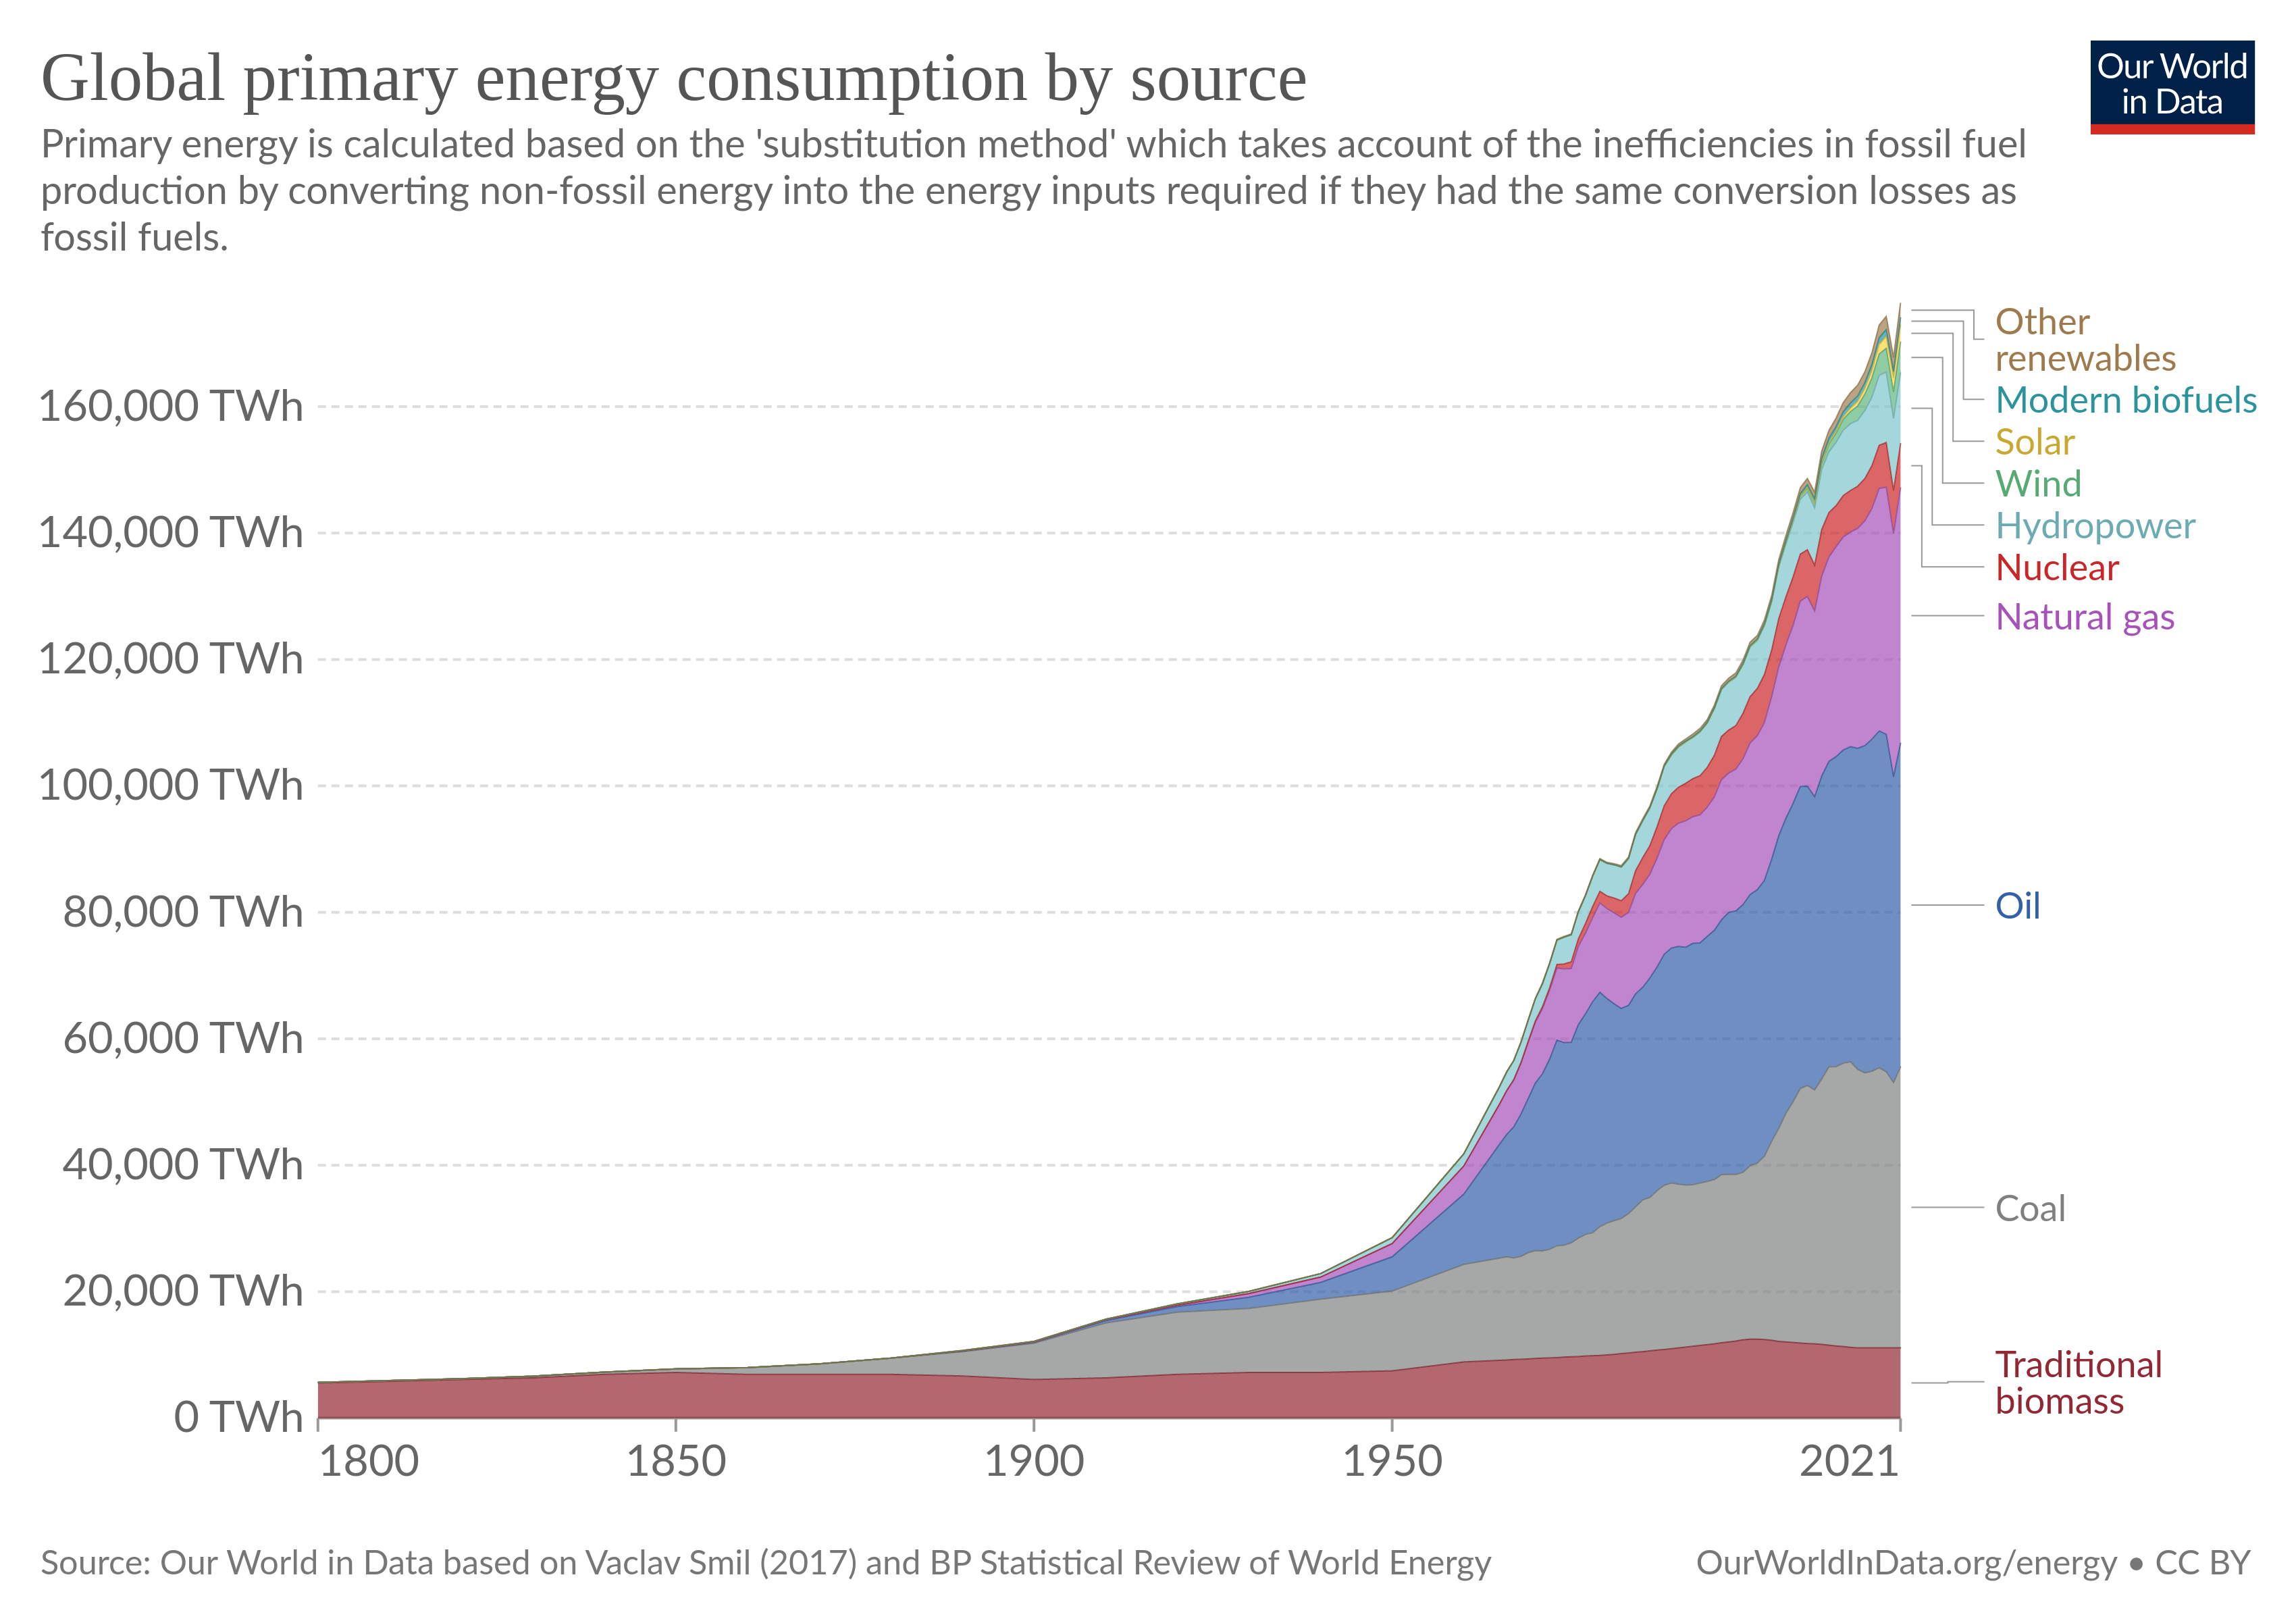
\includegraphics[width=\linewidth]{global_energy}
\end{frame}

\subsection{Law of Conservation of Energy}

\begin{frame}{Law of Conservation of Energy}
  \begin{center}
    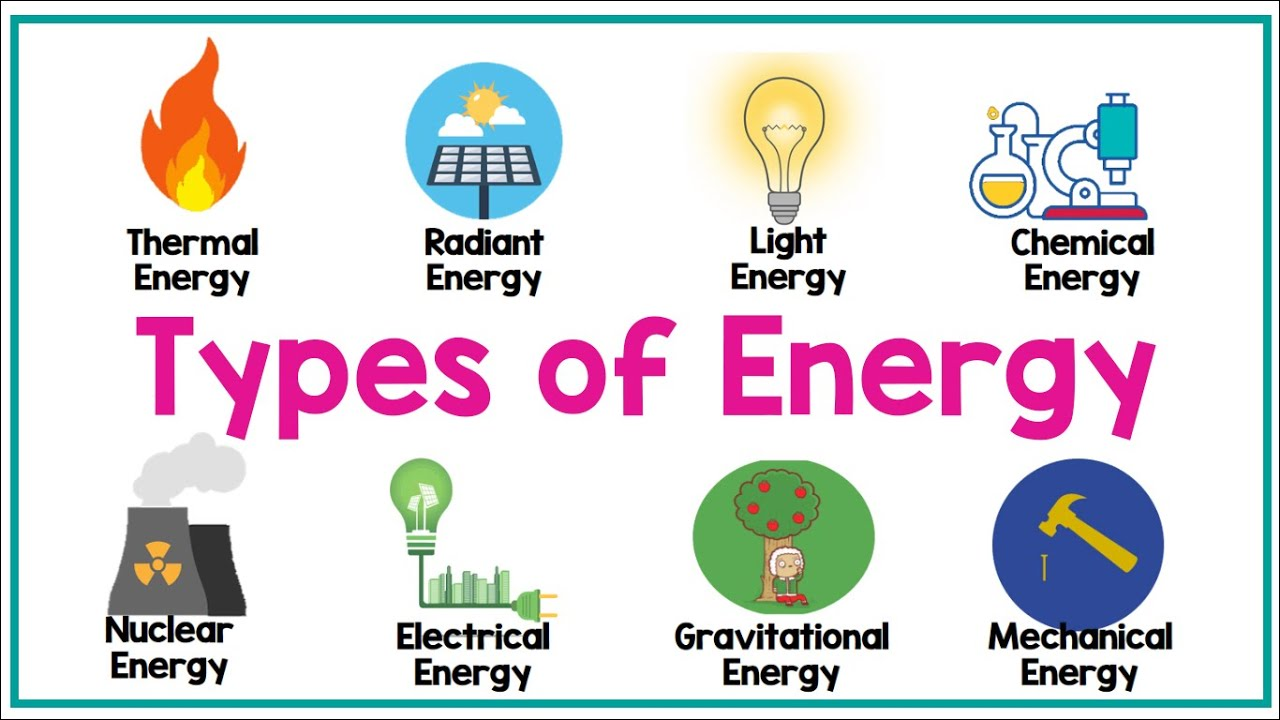
\includegraphics[scale=0.15]{energy_types}
    
    \textbf{Energy is neither created nor destroyed}
  \end{center}

  \begin{itemize}
  \item Energy can be converted from form to another
    e.g. mechanical, chemical, thermal, nuclear,
    electrical and vibrational energy
  \item Converting from one energy form to another is
    never $100\%$ efficient; there is always a loss of
    energy
  \end{itemize}
\end{frame}

\begin{frame}{Context: Energy Loss}
  \centering
  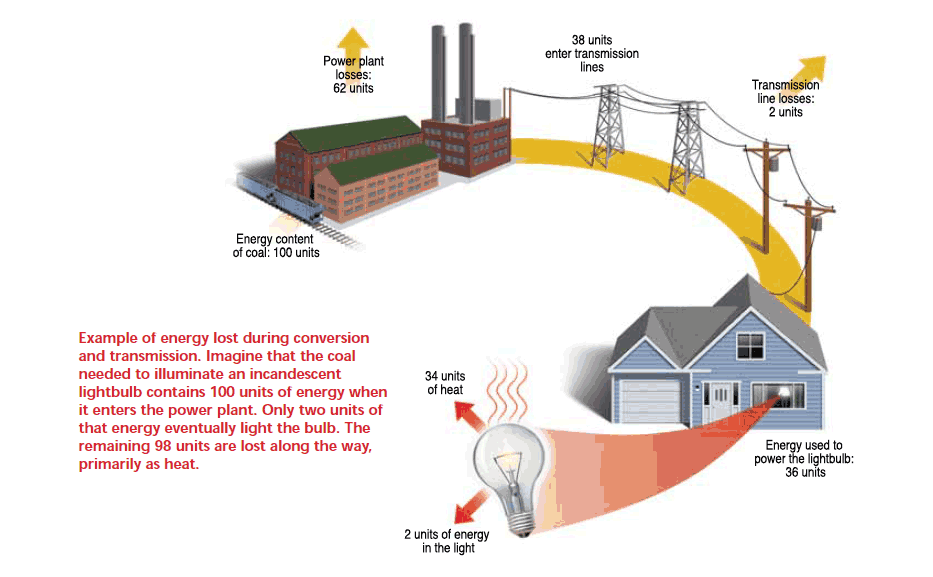
\includegraphics[width=0.9\linewidth]{energy_loss}

  Approximately only $\sim 30\%$ efficiency
\end{frame}

\subsection{Endothermic and Exothermic Reactions}

\begin{frame}{Endothermic and Exothermic Reactions}
  \centering
  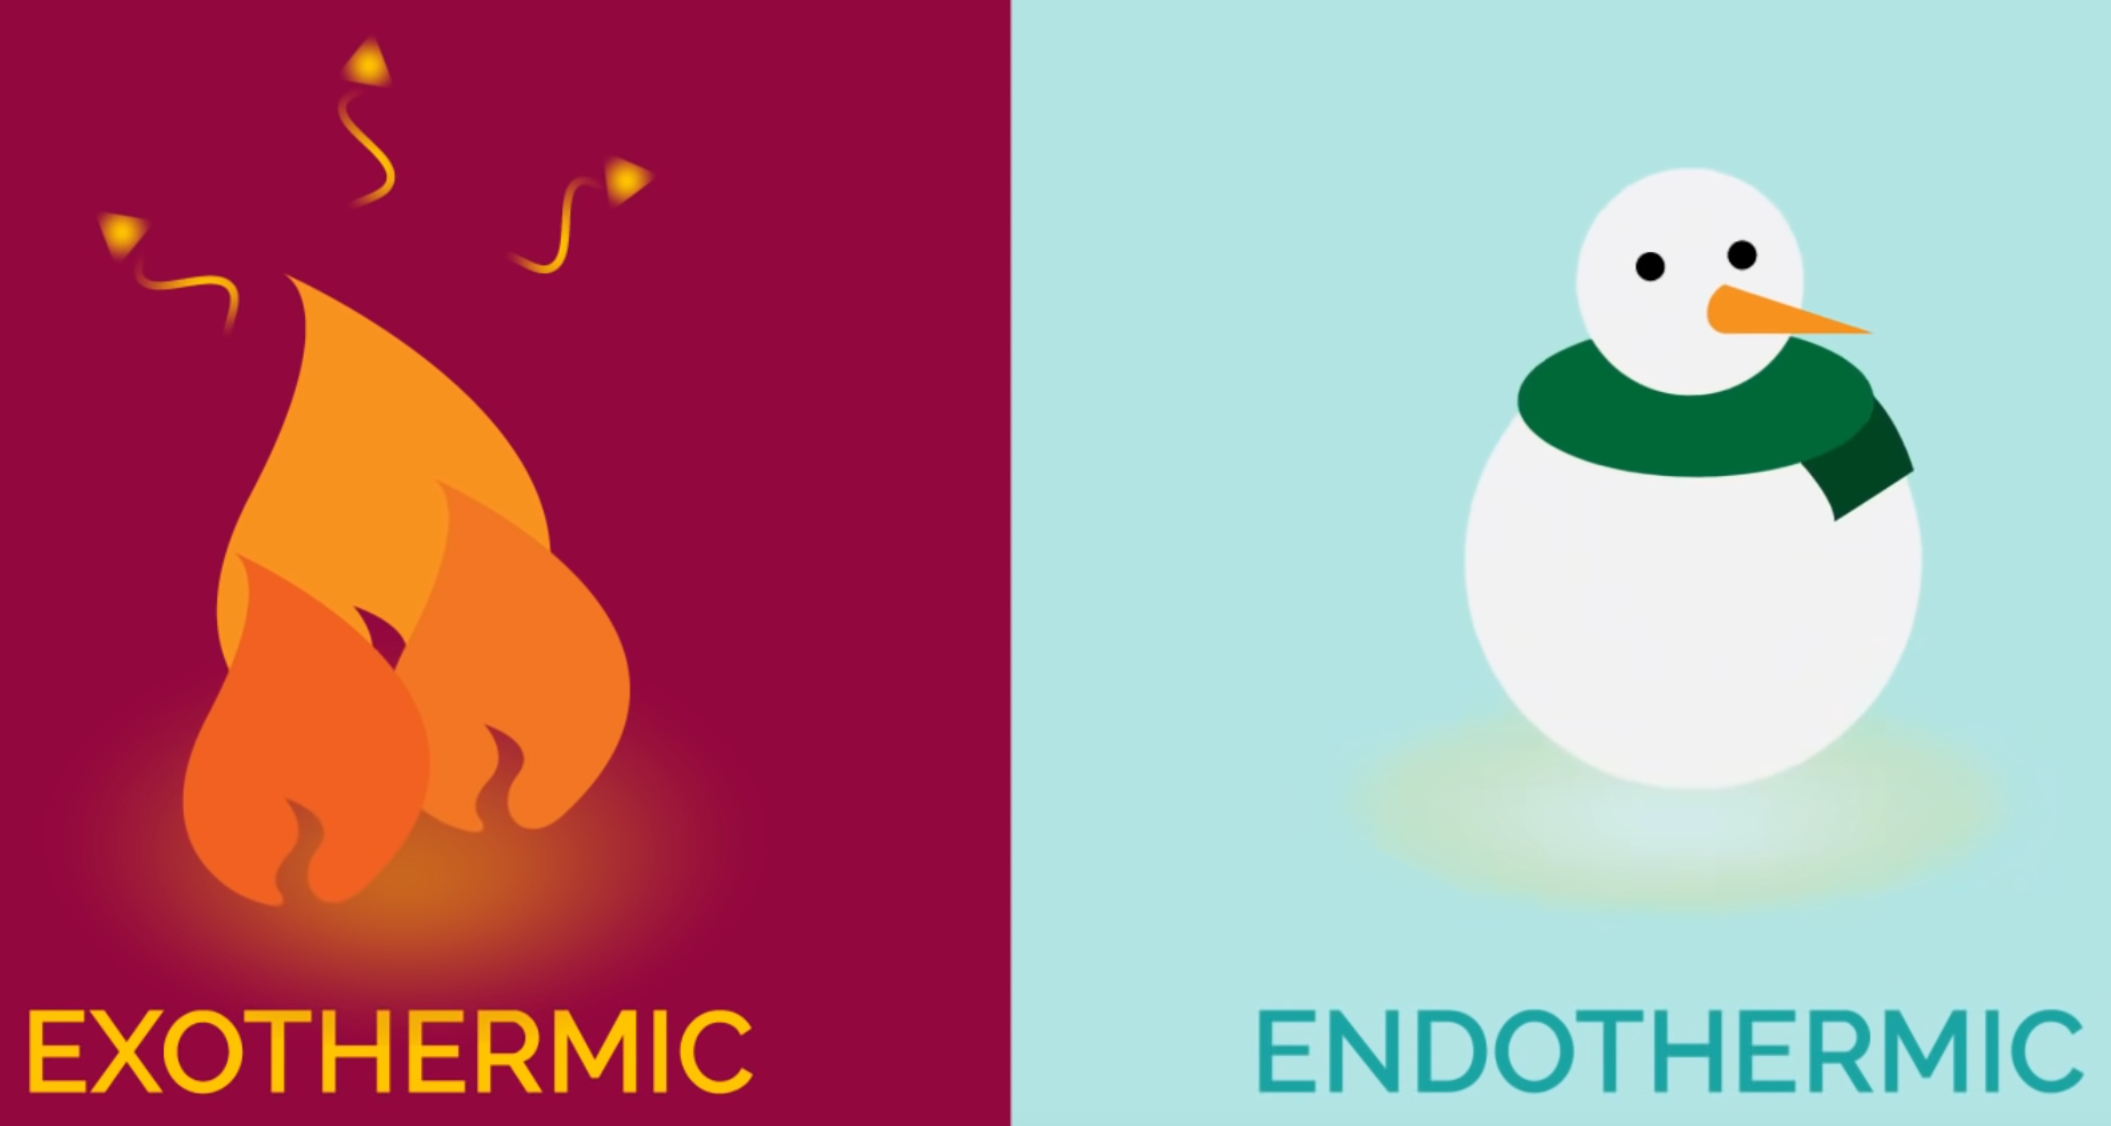
\includegraphics[width=0.8\linewidth]{exo_endo}

  \textbf{Exo} - external; exothermic reactions give off
  heat

  \textbf{Endo} - internal; endothermic reactions absorb
  heat
\end{frame}

\begin{frame}{Endothermic Reaction Diagram}
  \centering
  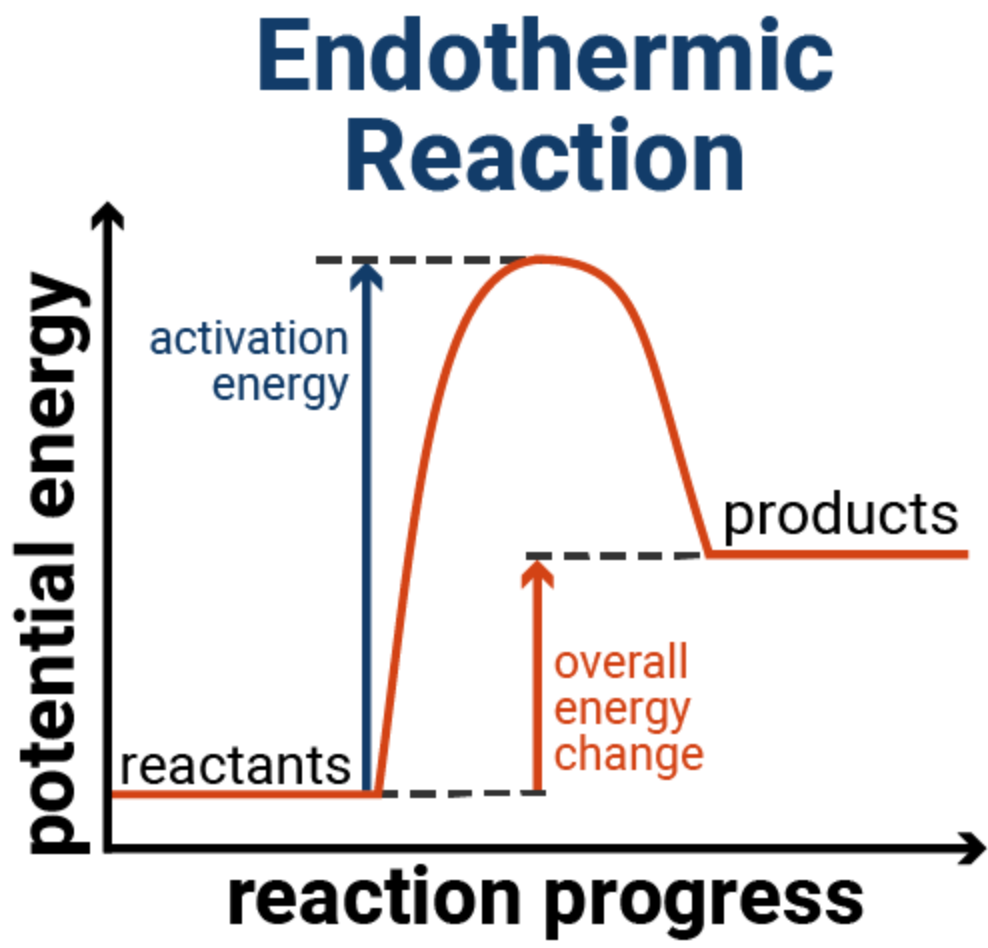
\includegraphics[width=0.5\linewidth]{endo_rxn}

  \begin{itemize}
  \item \textbf{Recall Potential energy} - ability to do
    work; $\Delta E_\text{products} > \Delta E_\text{reactants}$
  \item \textbf{Activation energy} - minimum energy to start the
    reaction; determines the rate at which the reaction undergoes
  \end{itemize}
\end{frame}

\begin{frame}{Examples of Endothermic Reactions}
  \centering
  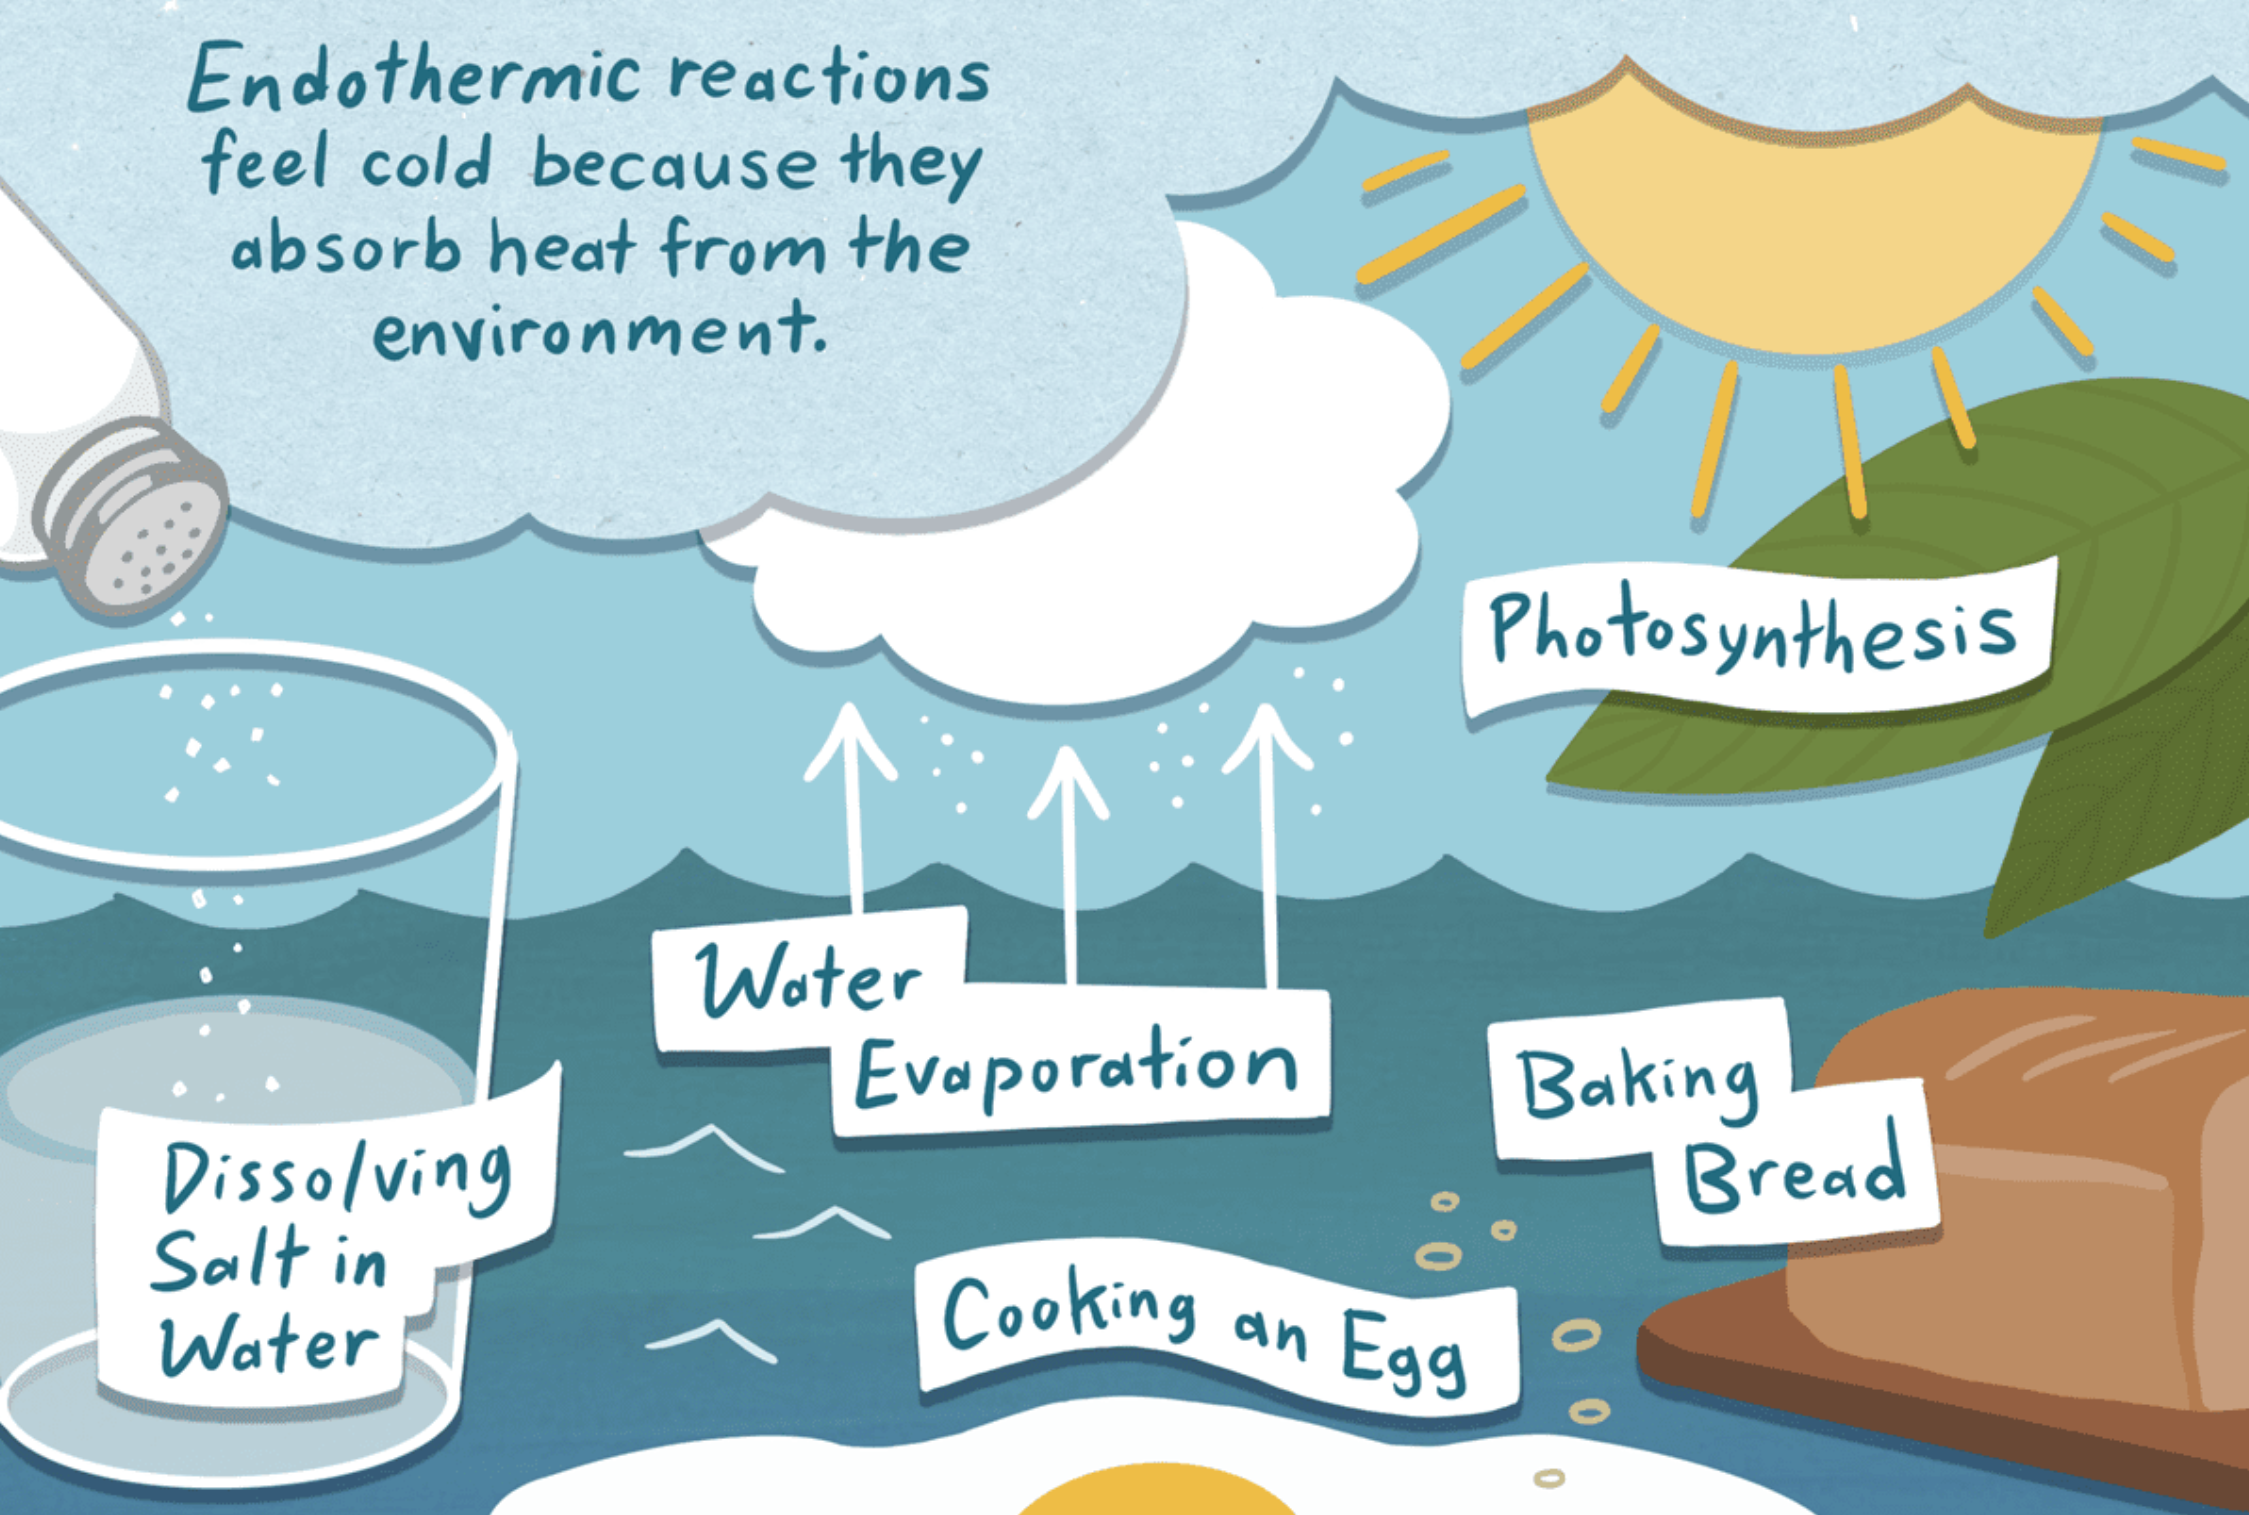
\includegraphics[width=\linewidth]{endo_everyday}
\end{frame}

\begin{frame}{Exothermic Reaction Diagram}
  \centering
  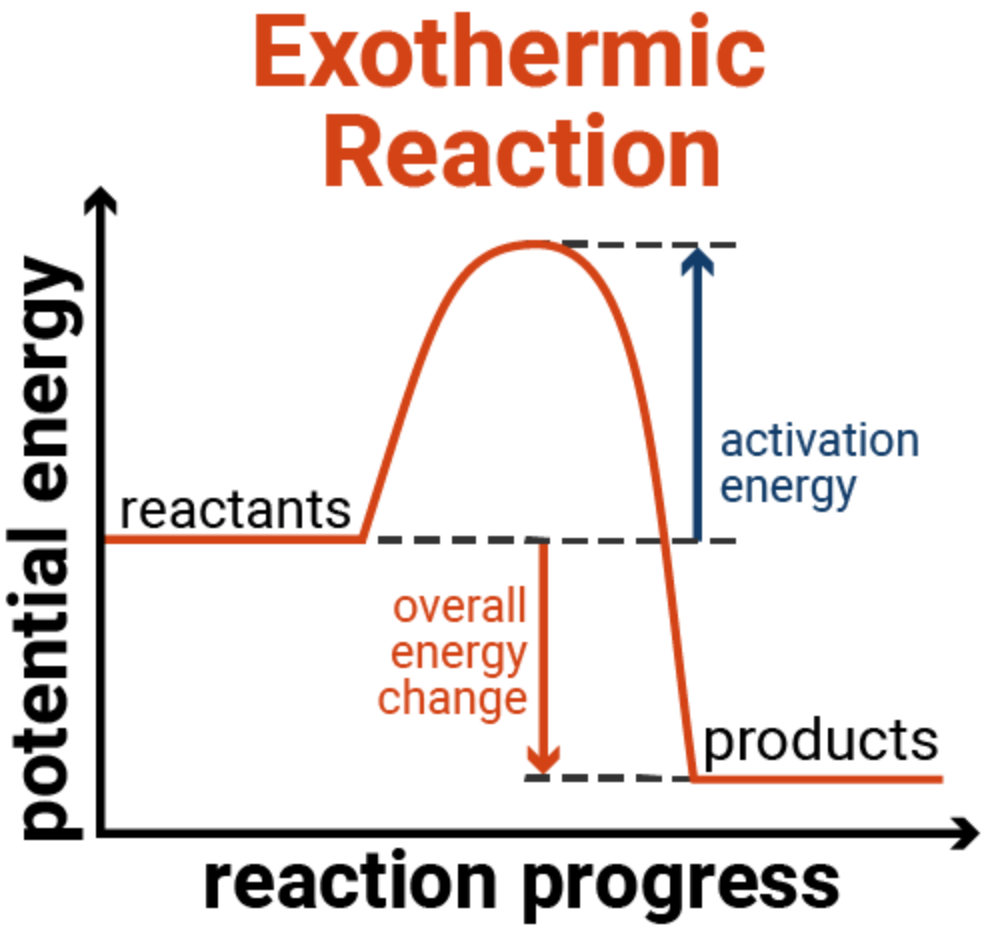
\includegraphics[width=0.5\linewidth]{exo_rxn}
  \begin{itemize}
  \item \textbf{Potential energy} - $\Delta E_\text{products} < \Delta E_\text{reactants}$
  \item Products are more stable than reactants since preference
    for lower energy state
  \end{itemize}
\end{frame}

\begin{frame}{Examples of Exothermic Reactions}
  \centering
  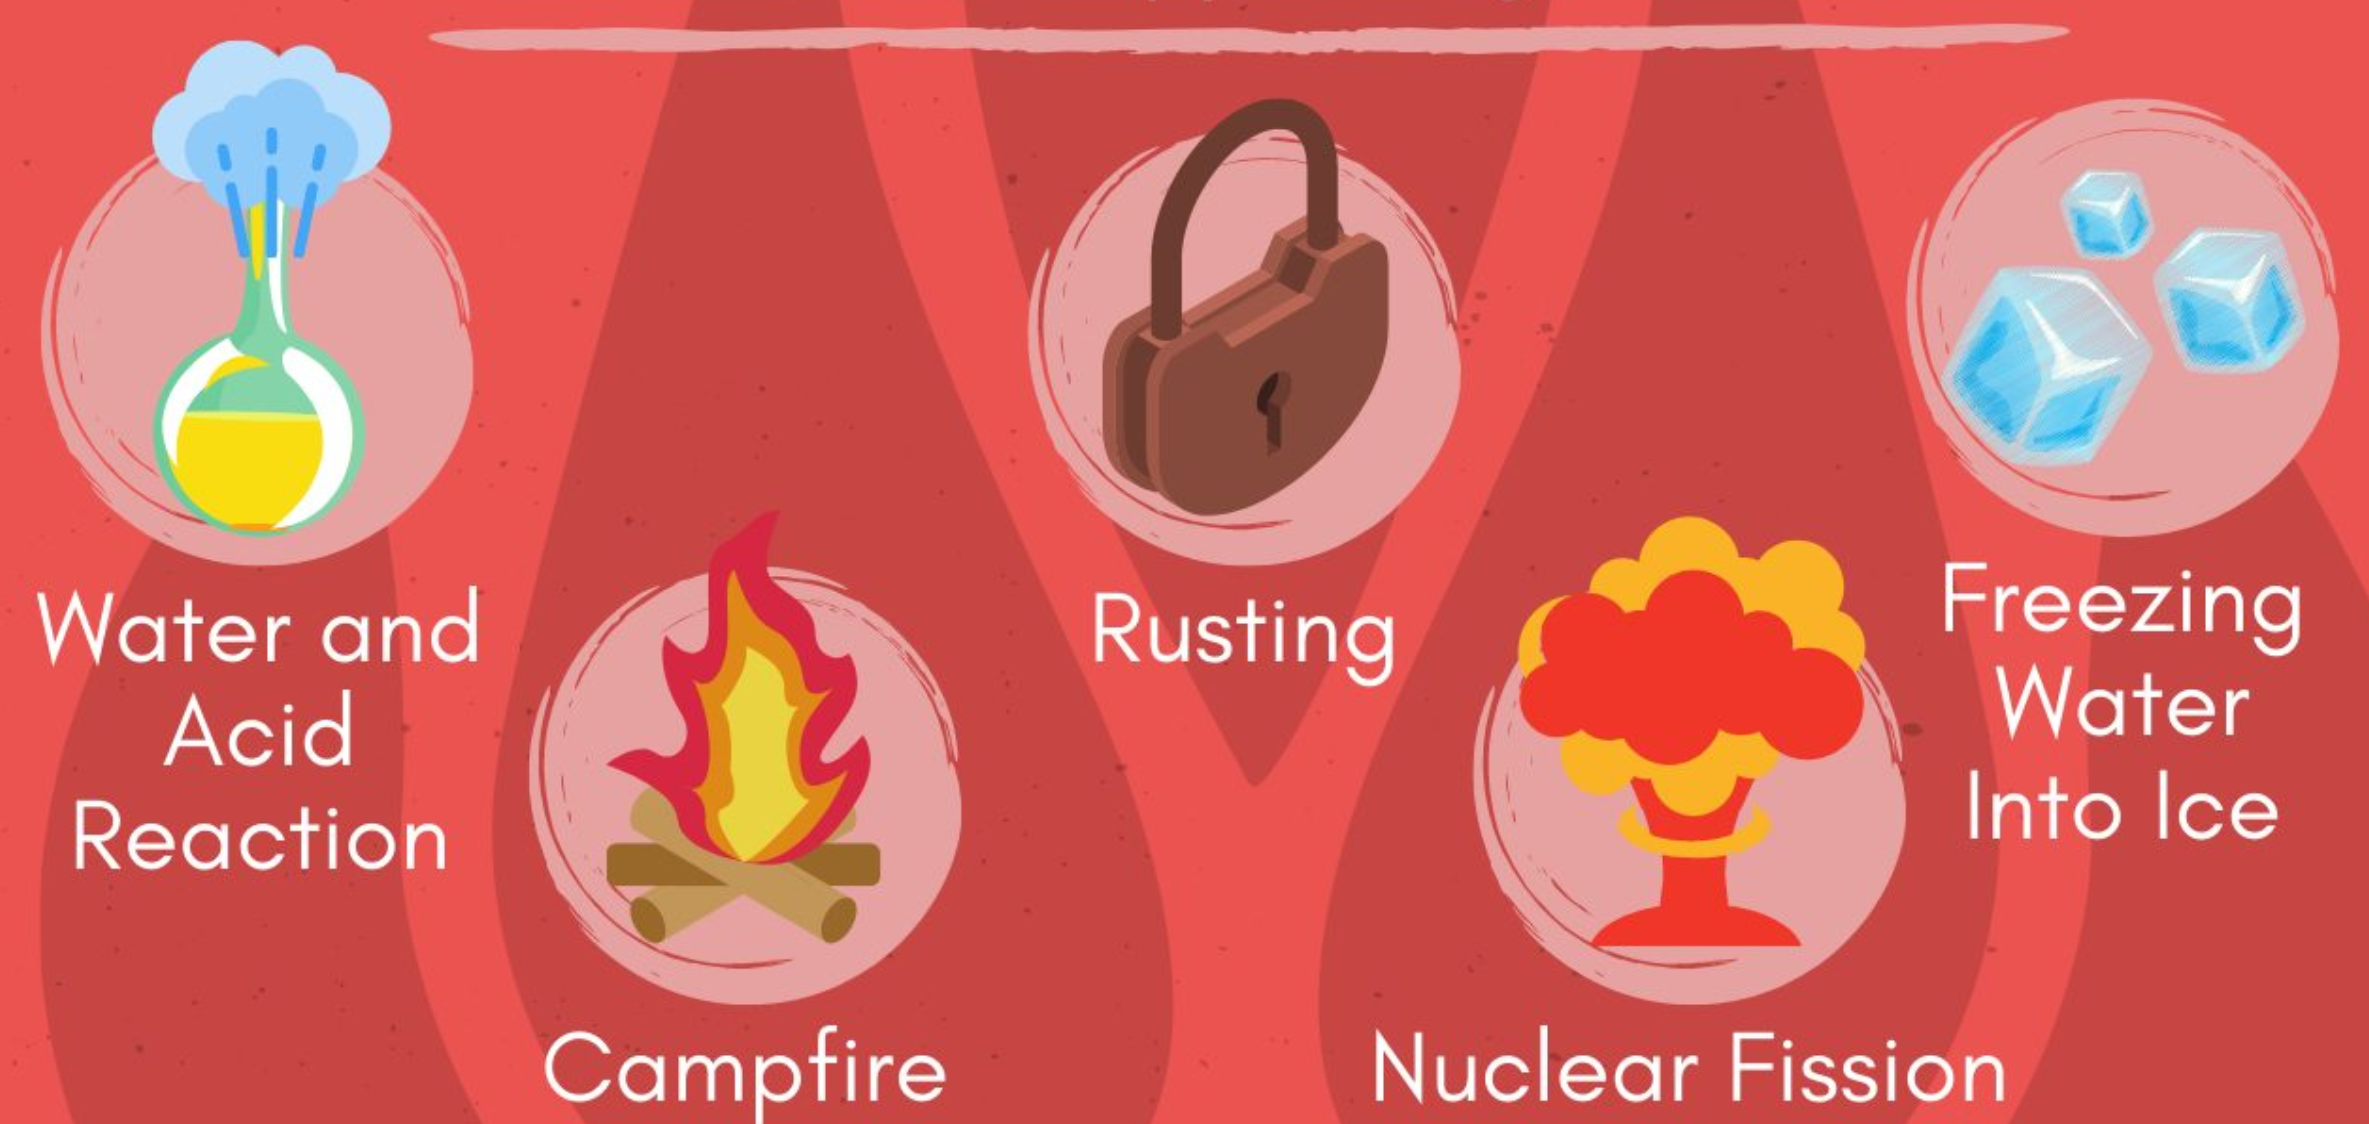
\includegraphics[width=\linewidth]{exo_everyday}
\end{frame}

\begin{frame}{Nuclear Fission}
  \centering
  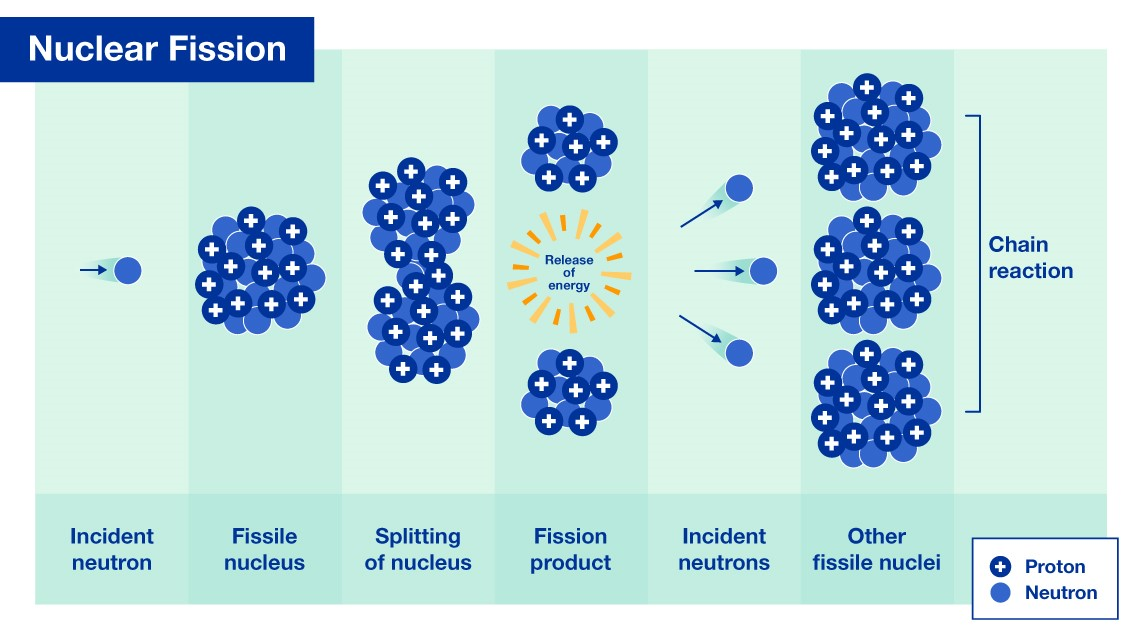
\includegraphics[width=0.8\linewidth]{nuclear_fission}

  \begin{itemize}
  \item \textbf{Nuclear fission} - releases energy where the
    nucleus of an atom splits into two or smaller nuclei
  \item U-235 atoms breaking down to release up to 200 million
    eV ($4.6\times 10^9$ kcal/mol)
  \item \textbf{Context} - 9.71 kcal/mol to boil water
  \end{itemize}
\end{frame}

\begin{frame}{Practice: Endothermic and Exothermic Reactions}
  Consider the following reaction:

  2H$_2$(g) + O$_2$(g) $\rightarrow$ 2H$_2$O(g)

  a) Is this reaction endothermic or exothermic?

  b) Is the reverse reaction endothermic or exothermic?

  c) For the products or reactants, which ones have the higher
  potential energy?

\end{frame}

\begin{frame}{Familiarize: Units of Energy}
  \centering
  4.184 J = 1 Cal

  \begin{itemize}
  \item ``Calories'' used on food items whould not be confused
    with the ``calorie'' used in chemistry
  \item 1 Cal = 1000 cal
  \end{itemize}
\end{frame}

\subsection{Calorimetry}

\begin{frame}{Calorimetry}
  \begin{columns}
    \column{0.3\textwidth}
    \begin{center}
      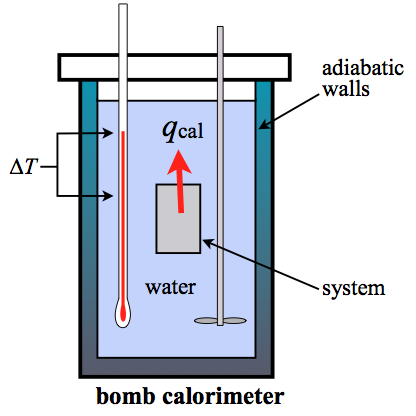
\includegraphics[scale=0.3]{bomb_calor}
    \end{center}
    \column{0.55\textwidth}
    \begin{equation}
      q = mC\Delta T
    \end{equation}
    where $q$ is heat, $m$ is the mass (g), $C$ is
    specific heat capacity ($^\circ$C/g) and $T$ is
    temperature ($^\circ$C)
  \end{columns}
  
  \begin{itemize}
  \item Performed at constant-pressure (atomospheric pressure)
  \item Bomb Calorimeter is Insulated where the heat evolved by the reaction
    is absorbed by the water
  \item \textbf{Specific Heat Capacity} - the amount of heat ($q$)
    required to heat an object 1$^\circ$C/g
  \end{itemize}
\end{frame}

\begin{frame}{Relating Conservation of Energy}
  \centering
  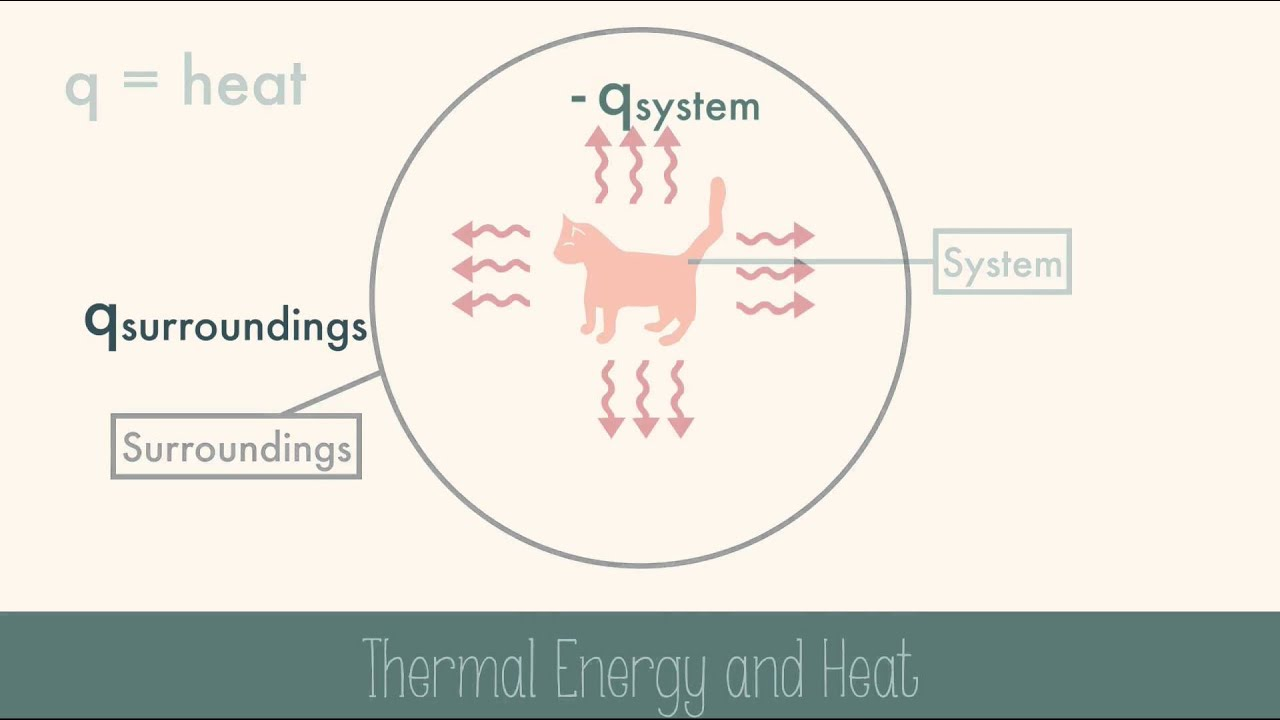
\includegraphics[width=0.8\textwidth]{heat_sys}

  $q_\text{system} + q_\text{surrounding} = 0$
  where $q$ is the heat

  Negative sign indicate released heat and positive sign indicates
  absorbed heat
\end{frame}

\begin{frame}{Example: Calorimetry}
  A brick is placed in an insulated calorimeter containing 5,000 kg of
  water. The temperature of the water decreases from 25.0$^\circ$C to
  19.4$^\circ$C when thermal equilibrium is reached

  a) Was the initial temperature of the brick greater than or less than
  the initial temperature of the water? Explain.

  b) What is the heat change $q$ of the brick? Specific heat capacity
  of water is 4.184 J/(g $^\circ$C).

  \vfill
\end{frame}

\begin{frame}{Practice: Heating Metal Alloy}
  A sample of metal alloy is heated and then placed in 125.0g of water
  held in a calorimeter at 22.5$^\circ$C. The final temperature of the water
  is 29.0$^\circ$C. Assume heat exchange only occurs between the water and alloy.

  a) Was the initial temperature of the alloy $>$ or $<$ the initial
  temperature of the water? Explain

  b) What is hte heat change of the alloy? Specific heat capacity
  of water is 4.184 J/(g $^\circ$C).

  \vfill
\end{frame}

\begin{frame}{Example: Relating to Chemical Reactions}
  Ethanol (CH$_3$CH$_2$OH) burns in excess oxygen. The heat change $q$
  for the reaction is $-1367$ kJ/mol.

  a) Is this reaction endothermic or exothermic?

  b) What is the heat change when 0.200 mol of CH$_3$CH$_2$OH burns?

  \onslide<2->{\textbf{a)} Exothermic}

  \onslide<3->{\textbf{b)}
    \begin{align*}
      0.200 \text{mol CH$_3$CH$_2$OH} \times \frac{-1367 \text{kJ}}{1 \text{mol CH$_3$CH$_2$OH}}
      = -273 \text{kJ}
    \end{align*}
  }
\end{frame}

\begin{frame}{Practice: Combination Reaction}
  Consider the combination reaction of hydrogen gas and solid
  iodine. The heat change $q$ for this reaction is $+53.00$ kJ/mol.

  a) Is this reaction endothermic or exothermic?

  b) What is the heat change when 2.50 mol of I$_2$ reacts?

  \vfill
\end{frame}

\end{document}
